\section{Data Overview and Preprocessing}

The exploratory data analysis began with an examination of the dataset structure and composition. The diabetic dataset comprises 101,766 patient encounters with 50 variables. 

The distribution of the target variable "readmitted" reveals that 54,864 (53.9\%) patients were not readmitted, 35,545 (34.9\%) were readmitted after 30 days, and 11,357 (11.2\%) were readmitted within 30 days (Figure 2.1).
The target variable is imbalanced, which is a common issue in healthcare datasets.

\begin{figure}[h]
    \centering
    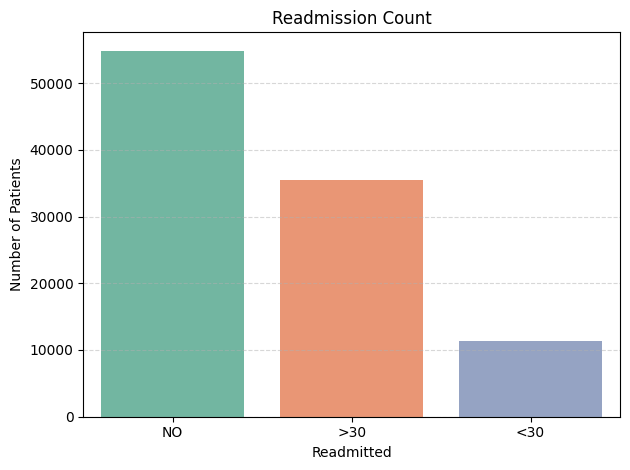
\includegraphics[width=0.7\textwidth]{../figures/readmission_distribution.png}
    \caption{Distribution of patient readmission categories}
    \label{fig:readmission_dist}
\end{figure}

Initial preprocessing steps included:
\begin{itemize}
    \item Removal of identifier variables (encounter\_id and patient\_nbr)
    \item Replacement of "?" placeholders with NaN values for proper missing value handling
\end{itemize}

\section{Missing Value Analysis and Imputation}

A critical aspect of the preprocessing phase involved identifying and addressing missing values within the dataset. 
Nine variables exhibited missing values, with "weight" showing the highest proportion at 96.9\%, followed by "max\_glu\_serum" and "A1Cresult" at 94.75\% and 83.28\% respectively.

\begin{figure}[h]
    \centering
    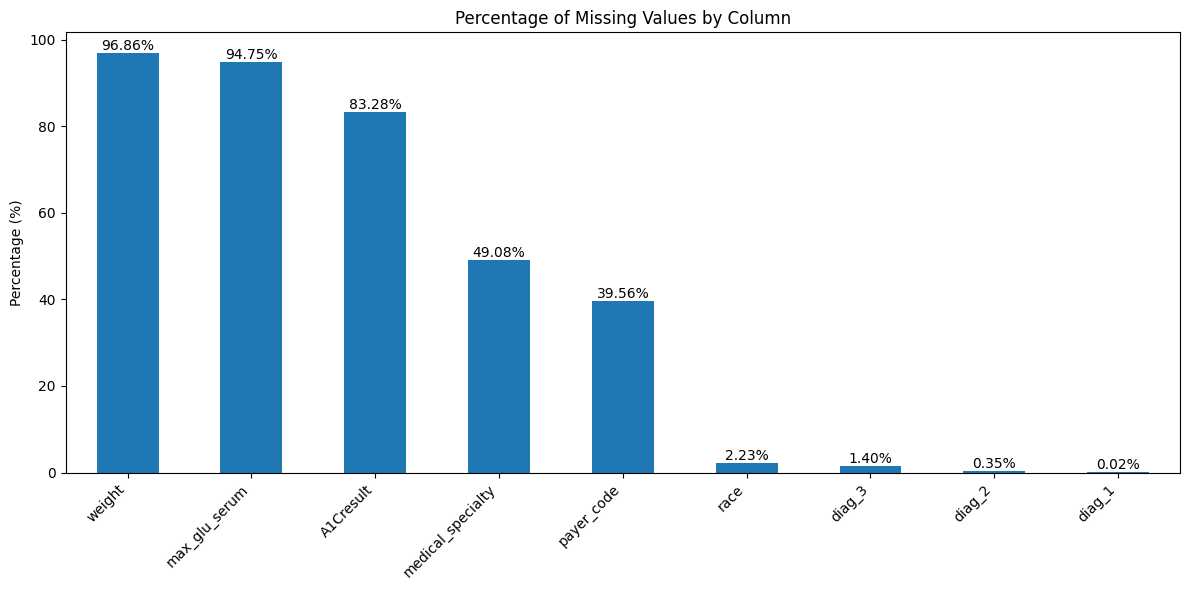
\includegraphics[width=0.8\textwidth]{../figures/missing_values_percentage.png}
    \caption{Percentage of missing values by variable}
    \label{fig:missing_values}
\end{figure}

The following imputation strategies were implemented:
\begin{itemize}
    \item Althought "weight" is very important factor to identify the diabete condition, however, due to its extremely high percentage of missing values (96.9\%) we dropped this variable.
    \item Despite its high percentage of missing values, due to small amount of categorical objects, the "max\_glu\_serum", "A1Cresult", and "medical\_specialty", were imputed with the value "None"
    \item Similar to the above categorical variables, the "payer\_code" and "race" variables were imputed with the value "None
    \item For diagnosis variables: "diag\_1", "diag\_2", "diag\_3", missing values were imputed with the value "None". Categories with less than 0.5\% occurrence were merged into a new "Rest" category to reduce dimensionality and prevent overfitting. 
    Due to its importance, the "diag\_1" variable was considered more important than "diag\_2", and "diag\_2" was considered more important than "diag\_3". If a patient has multiple diagnoses, the most important one was selected and put into the "diag" variable.
    The "Rest" category was created to handle the rare cases and thus has less importance ranking (after diag\_3).
    The "None" category was created to handle the missing values and has the least importance (after "Rest").
    This approach was used to handle the overfitting issue and reduce the dimensionality of the dataset.
    \item For "race", the missing values were imputed with "None", althought it could be algined with "Caucasian" or "AfricanAmerican" categories, due to high median values.
    \item For "age", the missing values were imputed with the median of the variable. ("age\_mid")
\end{itemize}

\section{Categorical Variable Analysis}

The dataset contains numerous categorical variables representing patient demographics, diagnoses, medications, and hospital admission details. Categorical variables were categorized into two groups based on their distribution patterns and relationship with the target variable.

\subsection{Key Categorical Variables}

Based on distribution analysis and correlation with the target variable, the following categorical variables were identified as significant:
\begin{itemize}
    \item Demographics: race, gender, payer\_code (Figure 2.3)
    \item Medical details: max\_glu\_serum, A1Cresult, medical\_specialty (Figure 2.4)
    \item Medications: metformin, glimepiride, glipizide, glyburide, pioglitazone, rosiglitazone (Figure 2.5)
    \item Treatment process: insulin,change, diabetesMed (Figure 2.6)
    \item Diagnosis: diag (Figure 2.7)
    \item Hospital factors: admission\_type\_id, discharge\_disposition\_id, admission\_source\_id (Figure 2.8)
\end{itemize}

\begin{figure}[h]
    \centering
    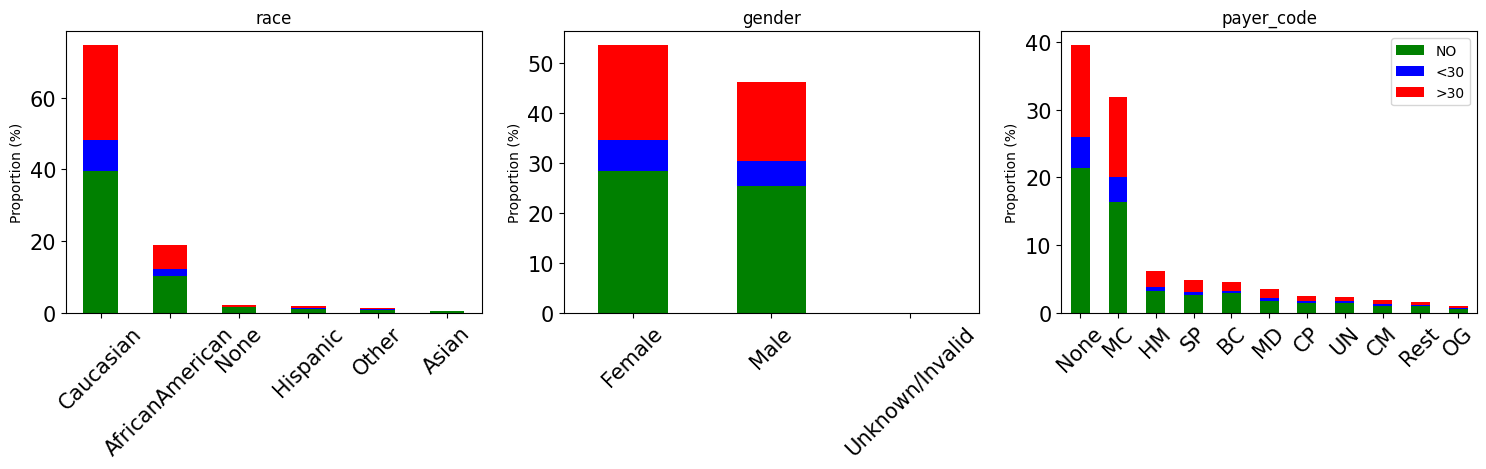
\includegraphics[width=0.9\textwidth]{../figures/cat1.png}
    \caption{Distribution of readmission status across Demographics}

    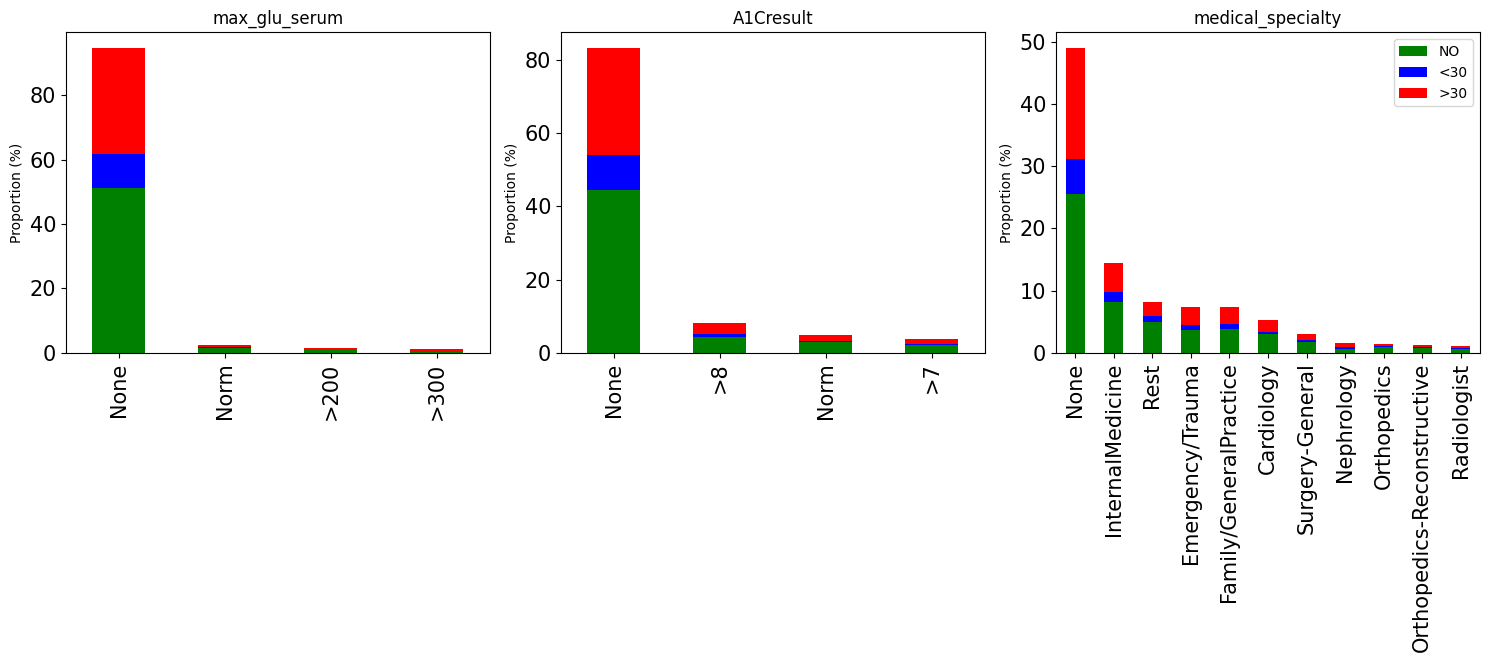
\includegraphics[width=0.9\textwidth]{../figures/cat2.png}
    \caption{Distribution of readmission status across Medical details}

    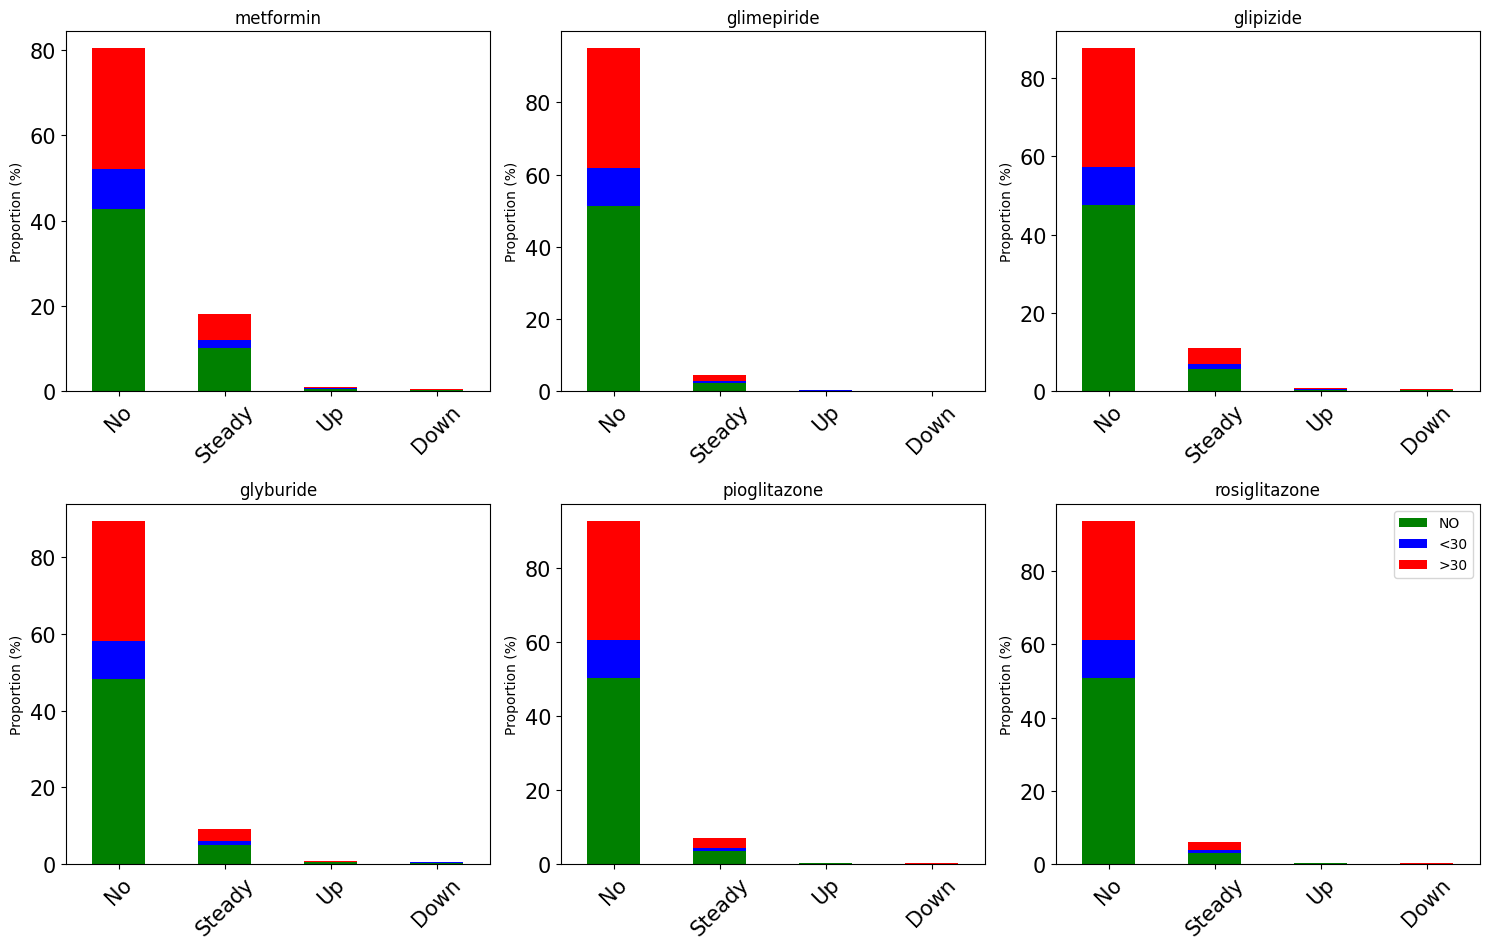
\includegraphics[width=0.9\textwidth]{../figures/cat3.png}
    \caption{Distribution of readmission status across Medications}
\end{figure}

\begin{figure}[h]
    \centering
    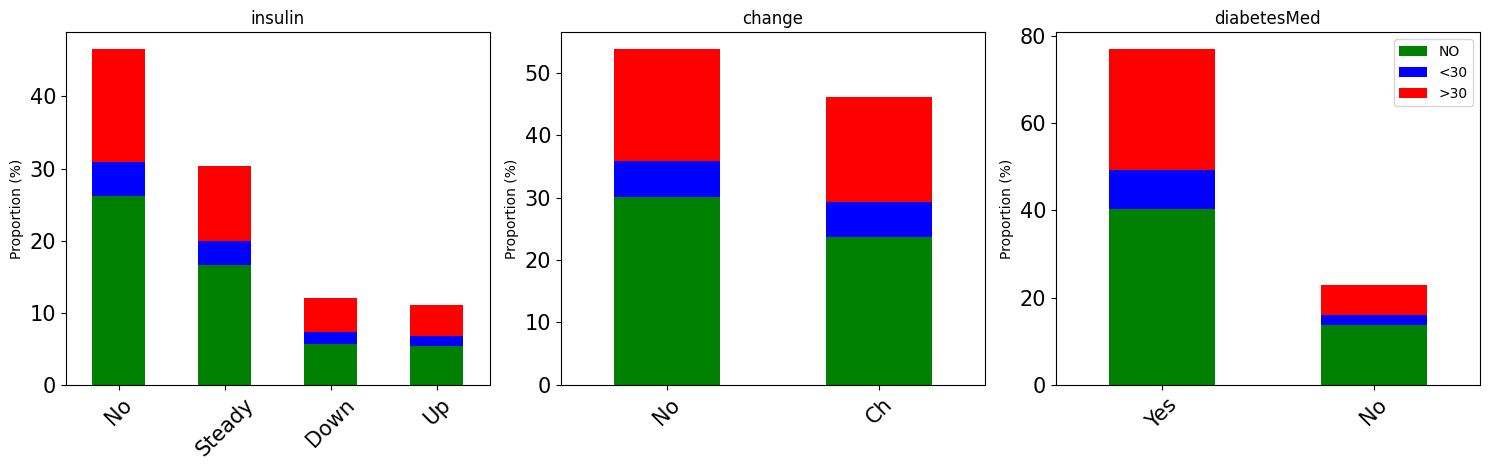
\includegraphics[width=0.9\textwidth]{../figures/cat4.png}
    \caption{Distribution of readmission status across Treatment process}

    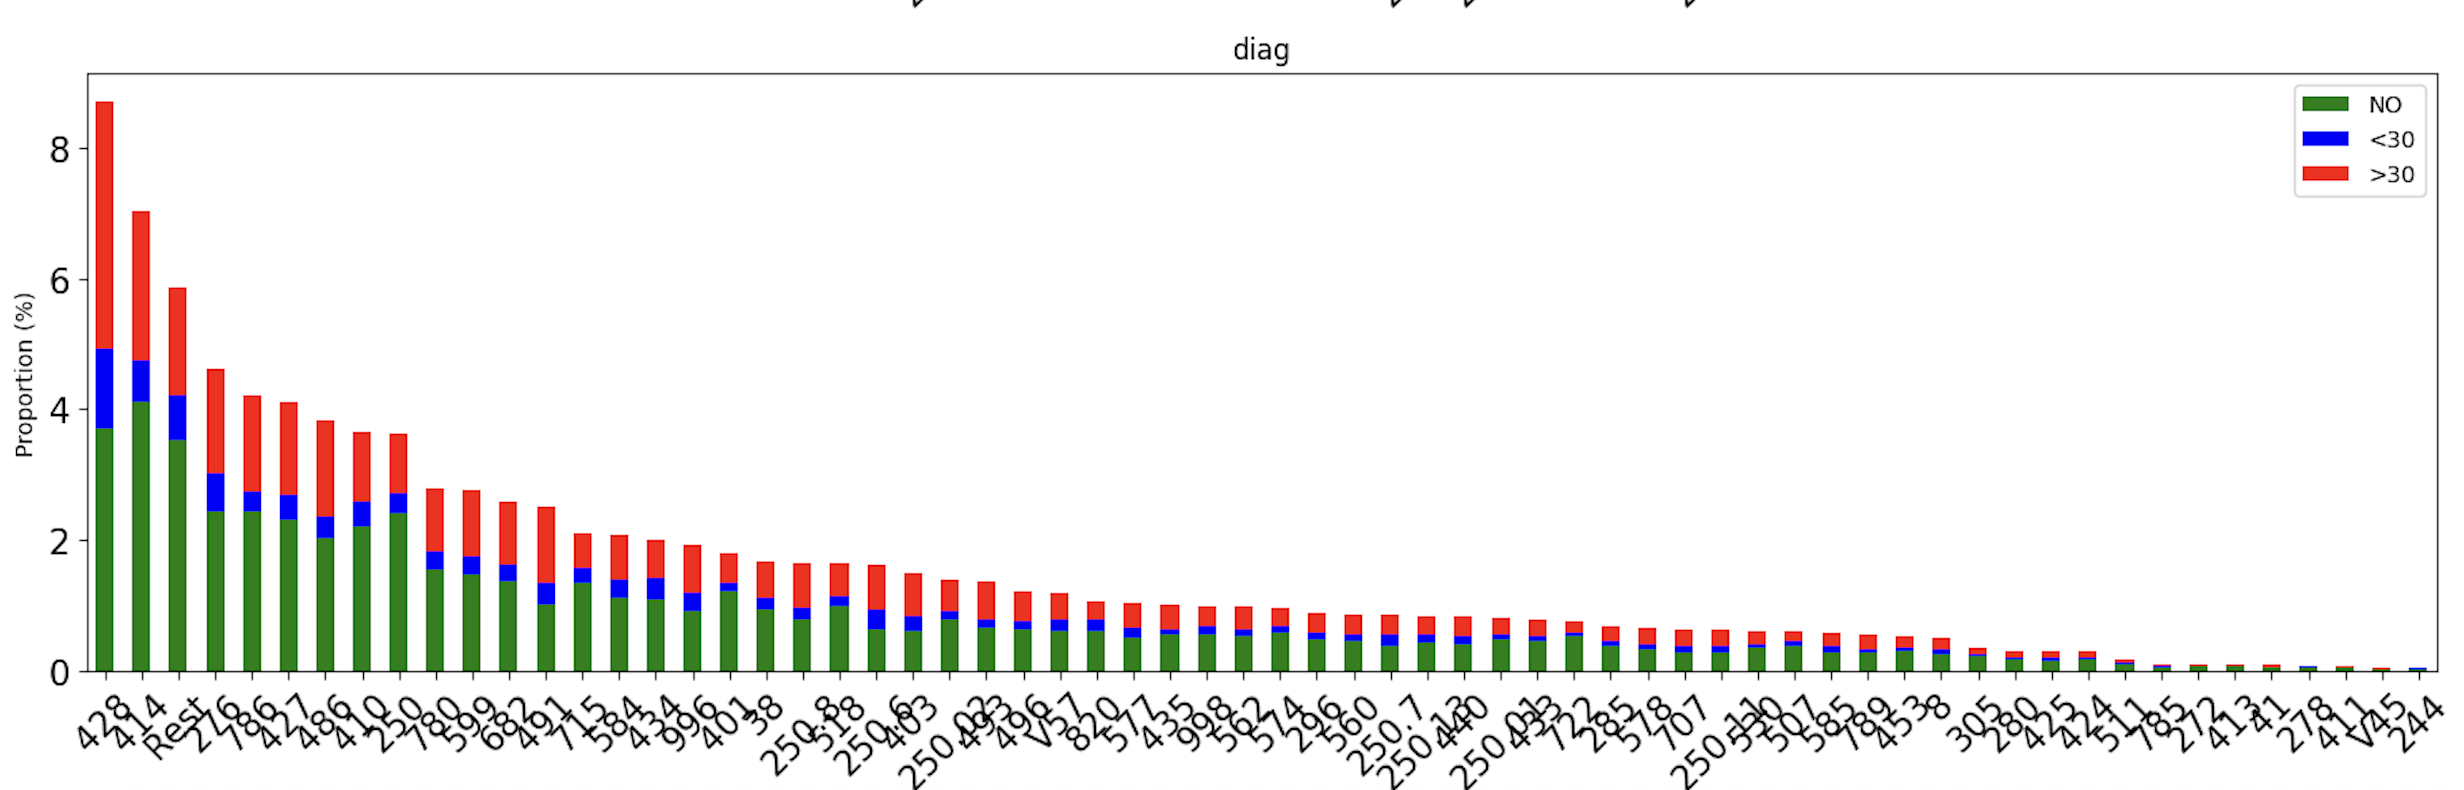
\includegraphics[width=0.9\textwidth]{../figures/cat5.png}
    \caption{Distribution of readmission status across Dignosis code}

    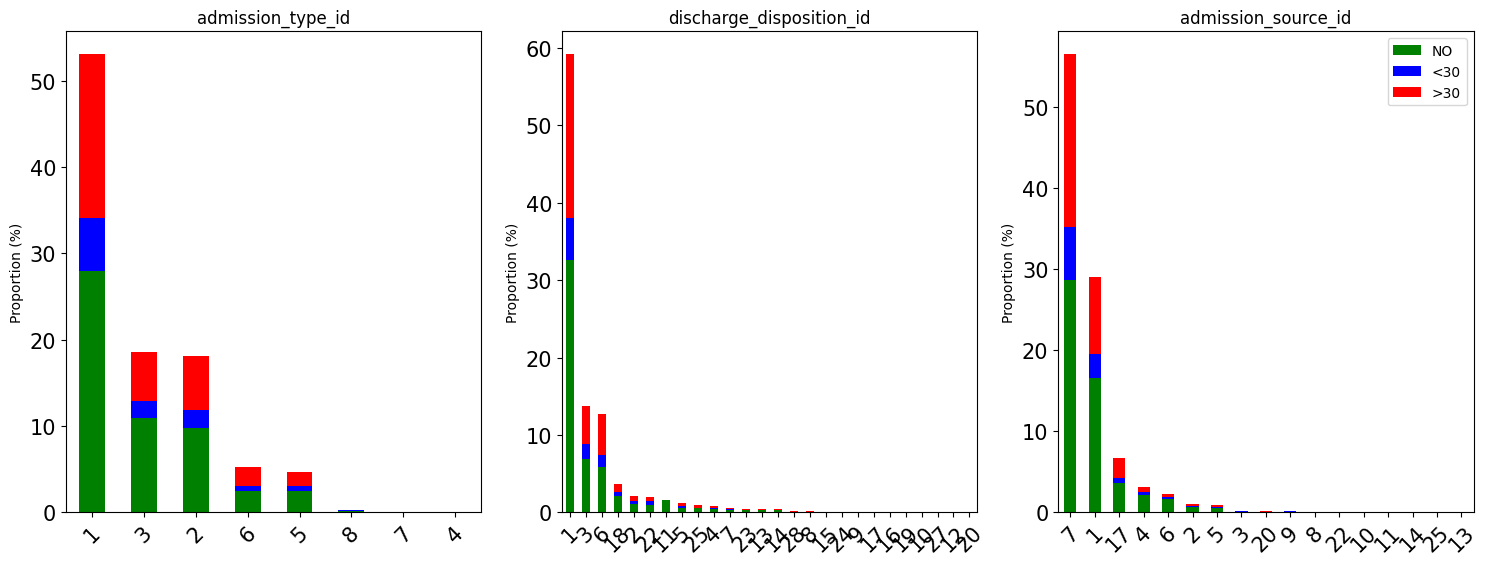
\includegraphics[width=0.9\textwidth]{../figures/cat6.png}
    \caption{Distribution of readmission status across Hospital factors}
    
\end{figure}

Notable findings include:
\begin{itemize}
    \item Race: Over 70\% of patients are Caucasian, with distinct readmission patterns across racial groups
    \item Admission type: Emergency intake (type 1) accounts for more than 50\% of admissions
    \item Discharge disposition: Approximately 60\% of patients are discharged to home
    \item Admission source: Nearly 60\% of admissions originate from emergency rooms, followed by 30\% from physician referrals
\end{itemize}



\subsection{Excluded Categorical Variables}

Several medication variables were excluded from further analysis due to extreme skewness that could lead to overfitting:
\begin{itemize}
    \item repalinize, nateglinide, chloropropamite, acetohesamide, tolbutamide
    \item acarbose, miglitol, troglitazone, tolazamide, examide
    \item citoglipton, gliburide\_metoformin, glipizide\_metoformin
    \item gplipiride\_glitopetazone, troglitazone, metorformin\_piglitazone
\end{itemize}

\section{Numerical Variable Analysis}

The numerical variables in the dataset include:
\begin{itemize}
    \item time\_in\_hospital: Length of hospital stay
    \item num\_lab\_procedures: Number of laboratory procedures
    \item num\_procedures: Number of procedures other than laboratory
    \item num\_medications: Number of distinct medications
    \item number\_outpatient: Number of outpatient visits
    \item number\_emergency: Number of emergency visits
    \item number\_inpatient: Number of inpatient visits
    \item number\_diagnoses: Number of diagnoses
    \item age\_mid: Midpoint of age range
\end{itemize}

\subsection{Correlation Analysis}

Correlation analysis was conducted to identify potential relationships between numerical variables. The correlation matrix did not reveal high collinearity between the variables, with most correlation coefficients below 0.4.

\begin{figure}[h]
    \centering
    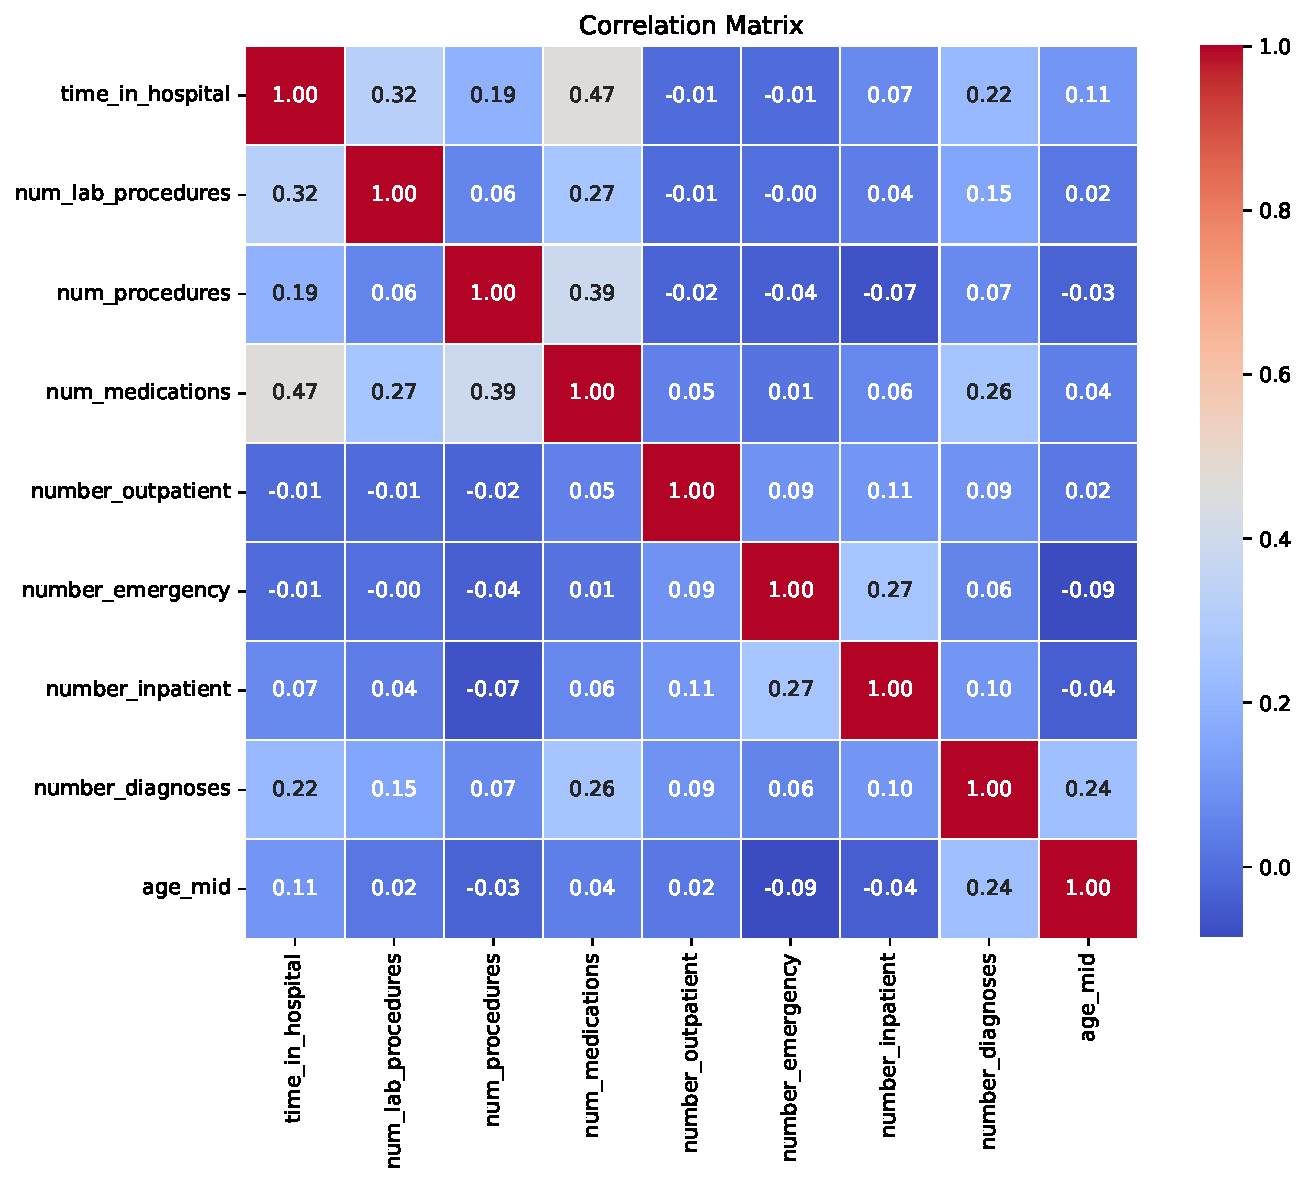
\includegraphics[width=0.8\textwidth]{../figures/correlation_matrix.pdf}
    \caption{Correlation matrix of numerical variables}
    \label{fig:corr_matrix}
\end{figure}

Variance Inflation Factor (VIF) analysis was also performed to detect multicollinearity. Although some potential collinearity was observed between "number\_diagnoses" and "age", the VIF values remained within acceptable ranges, and no variables were removed based on this analysis.

\begin{figure}[h]
    \centering
    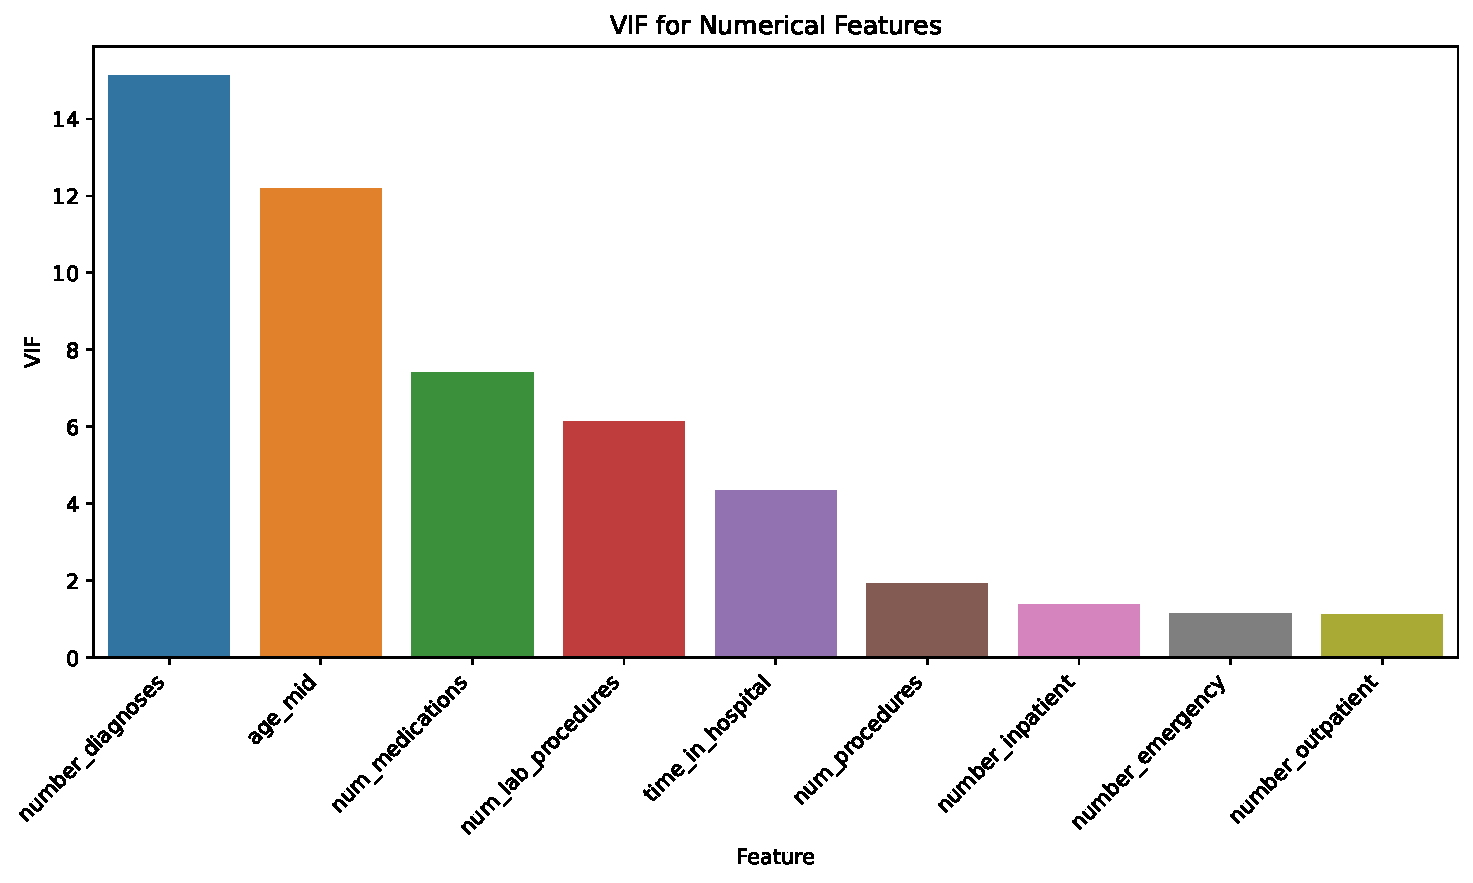
\includegraphics[width=0.8\textwidth]{../figures/vif_barplot.pdf}
    \caption{Variance Inflation Factor for numerical features}
    \label{fig:vif_barplot}
\end{figure}

\subsection{Distribution Analysis}

Distribution analysis of numerical variables revealed:
\begin{itemize}
    \item Right-skewed distributions for time\_in\_hospital
    \item Left-skewed distribution for age
    \item Extreme right-skew for number\_outpatient, number\_emergency, and number\_inpatient, with most values being zero
\end{itemize}

\begin{figure}[h]
    \centering
    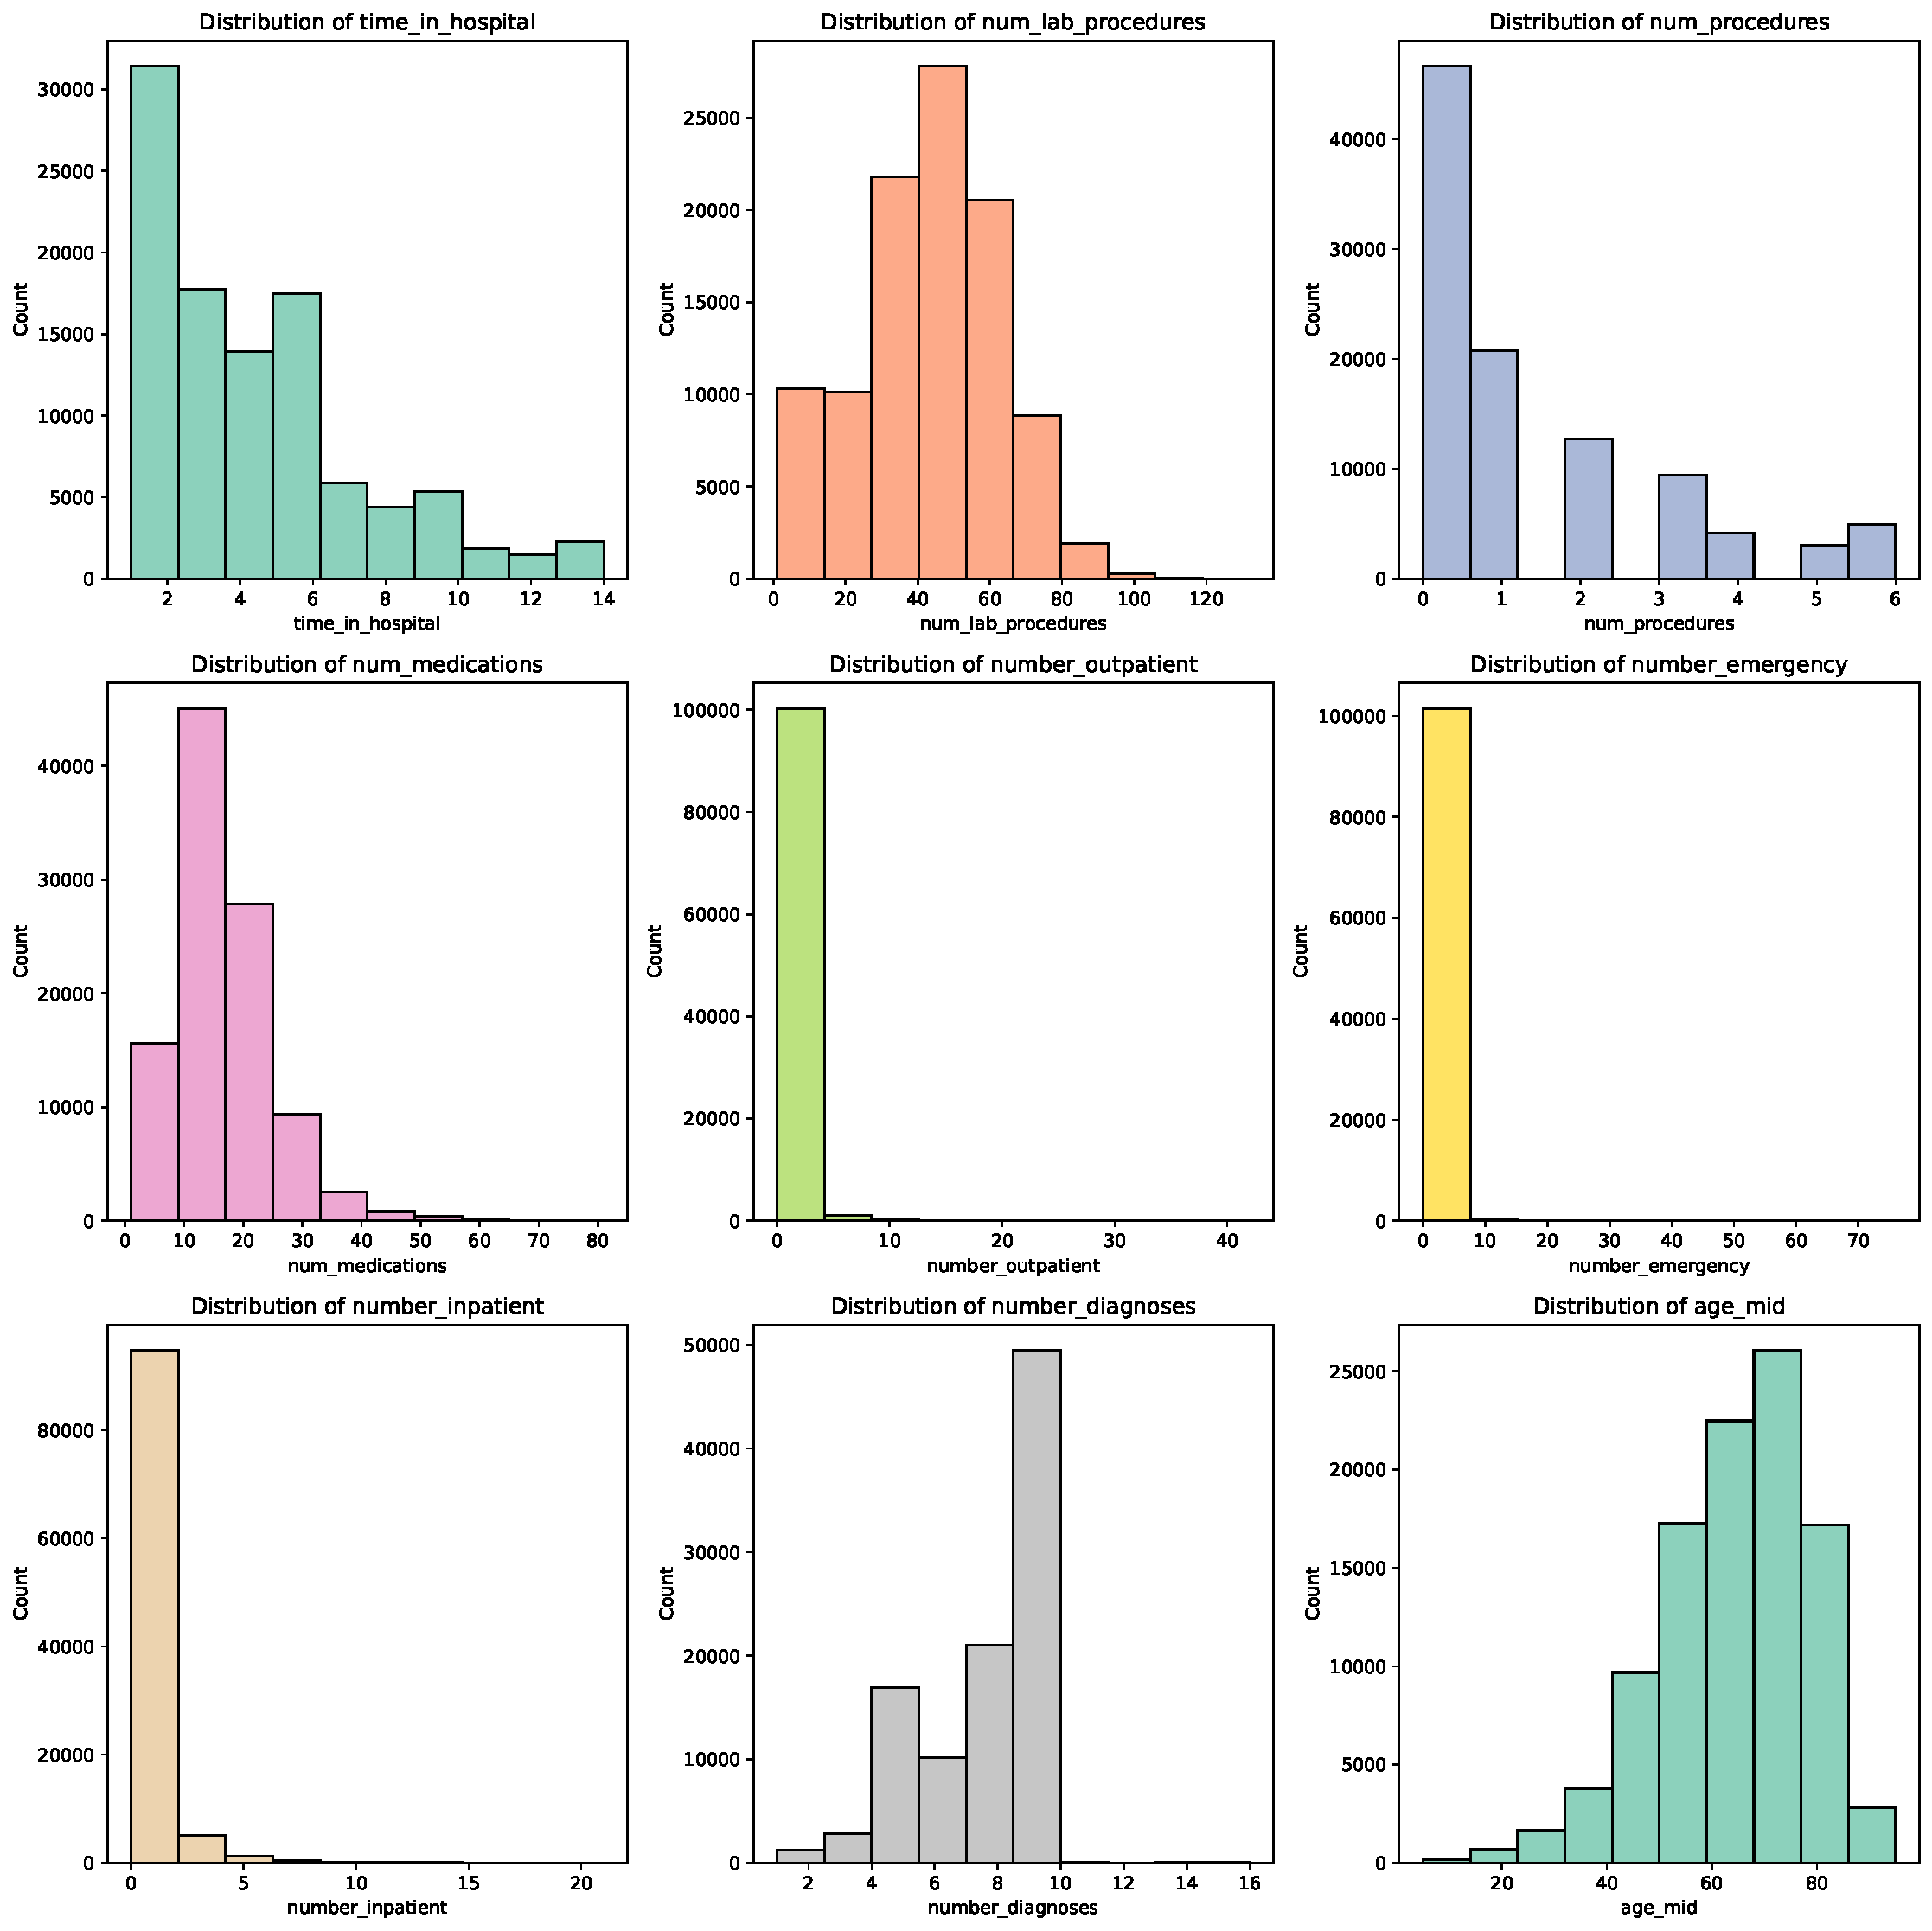
\includegraphics[width=0.9\textwidth]{../figures/numerical_distributions.pdf}
    \caption{Distribution of numerical variables}
    \label{fig:num_dist}
\end{figure}

Due to the extreme skew in outpatient, emergency, and inpatient visit counts, these variables were transformed into categorical variables:
\begin{itemize}
    \item cat\_outpatient: 0 for no visits, 1 for one or more visits
    \item cat\_emergency: 0 for no visits, 1 for one or more visits
    \item cat\_inpatient: 0 for no visits, 1 for one visit, 2 for more than one visit
\end{itemize}

\subsection{Relationship with Target Variable}

Boxplots were used to visualize the relationship between numerical variables and the readmission status. The analysis showed comparable distributions across the three readmission categories, indicating that standardization of numerical variables would be appropriate before integration with categorical features.

\begin{figure}[h]
    \centering
    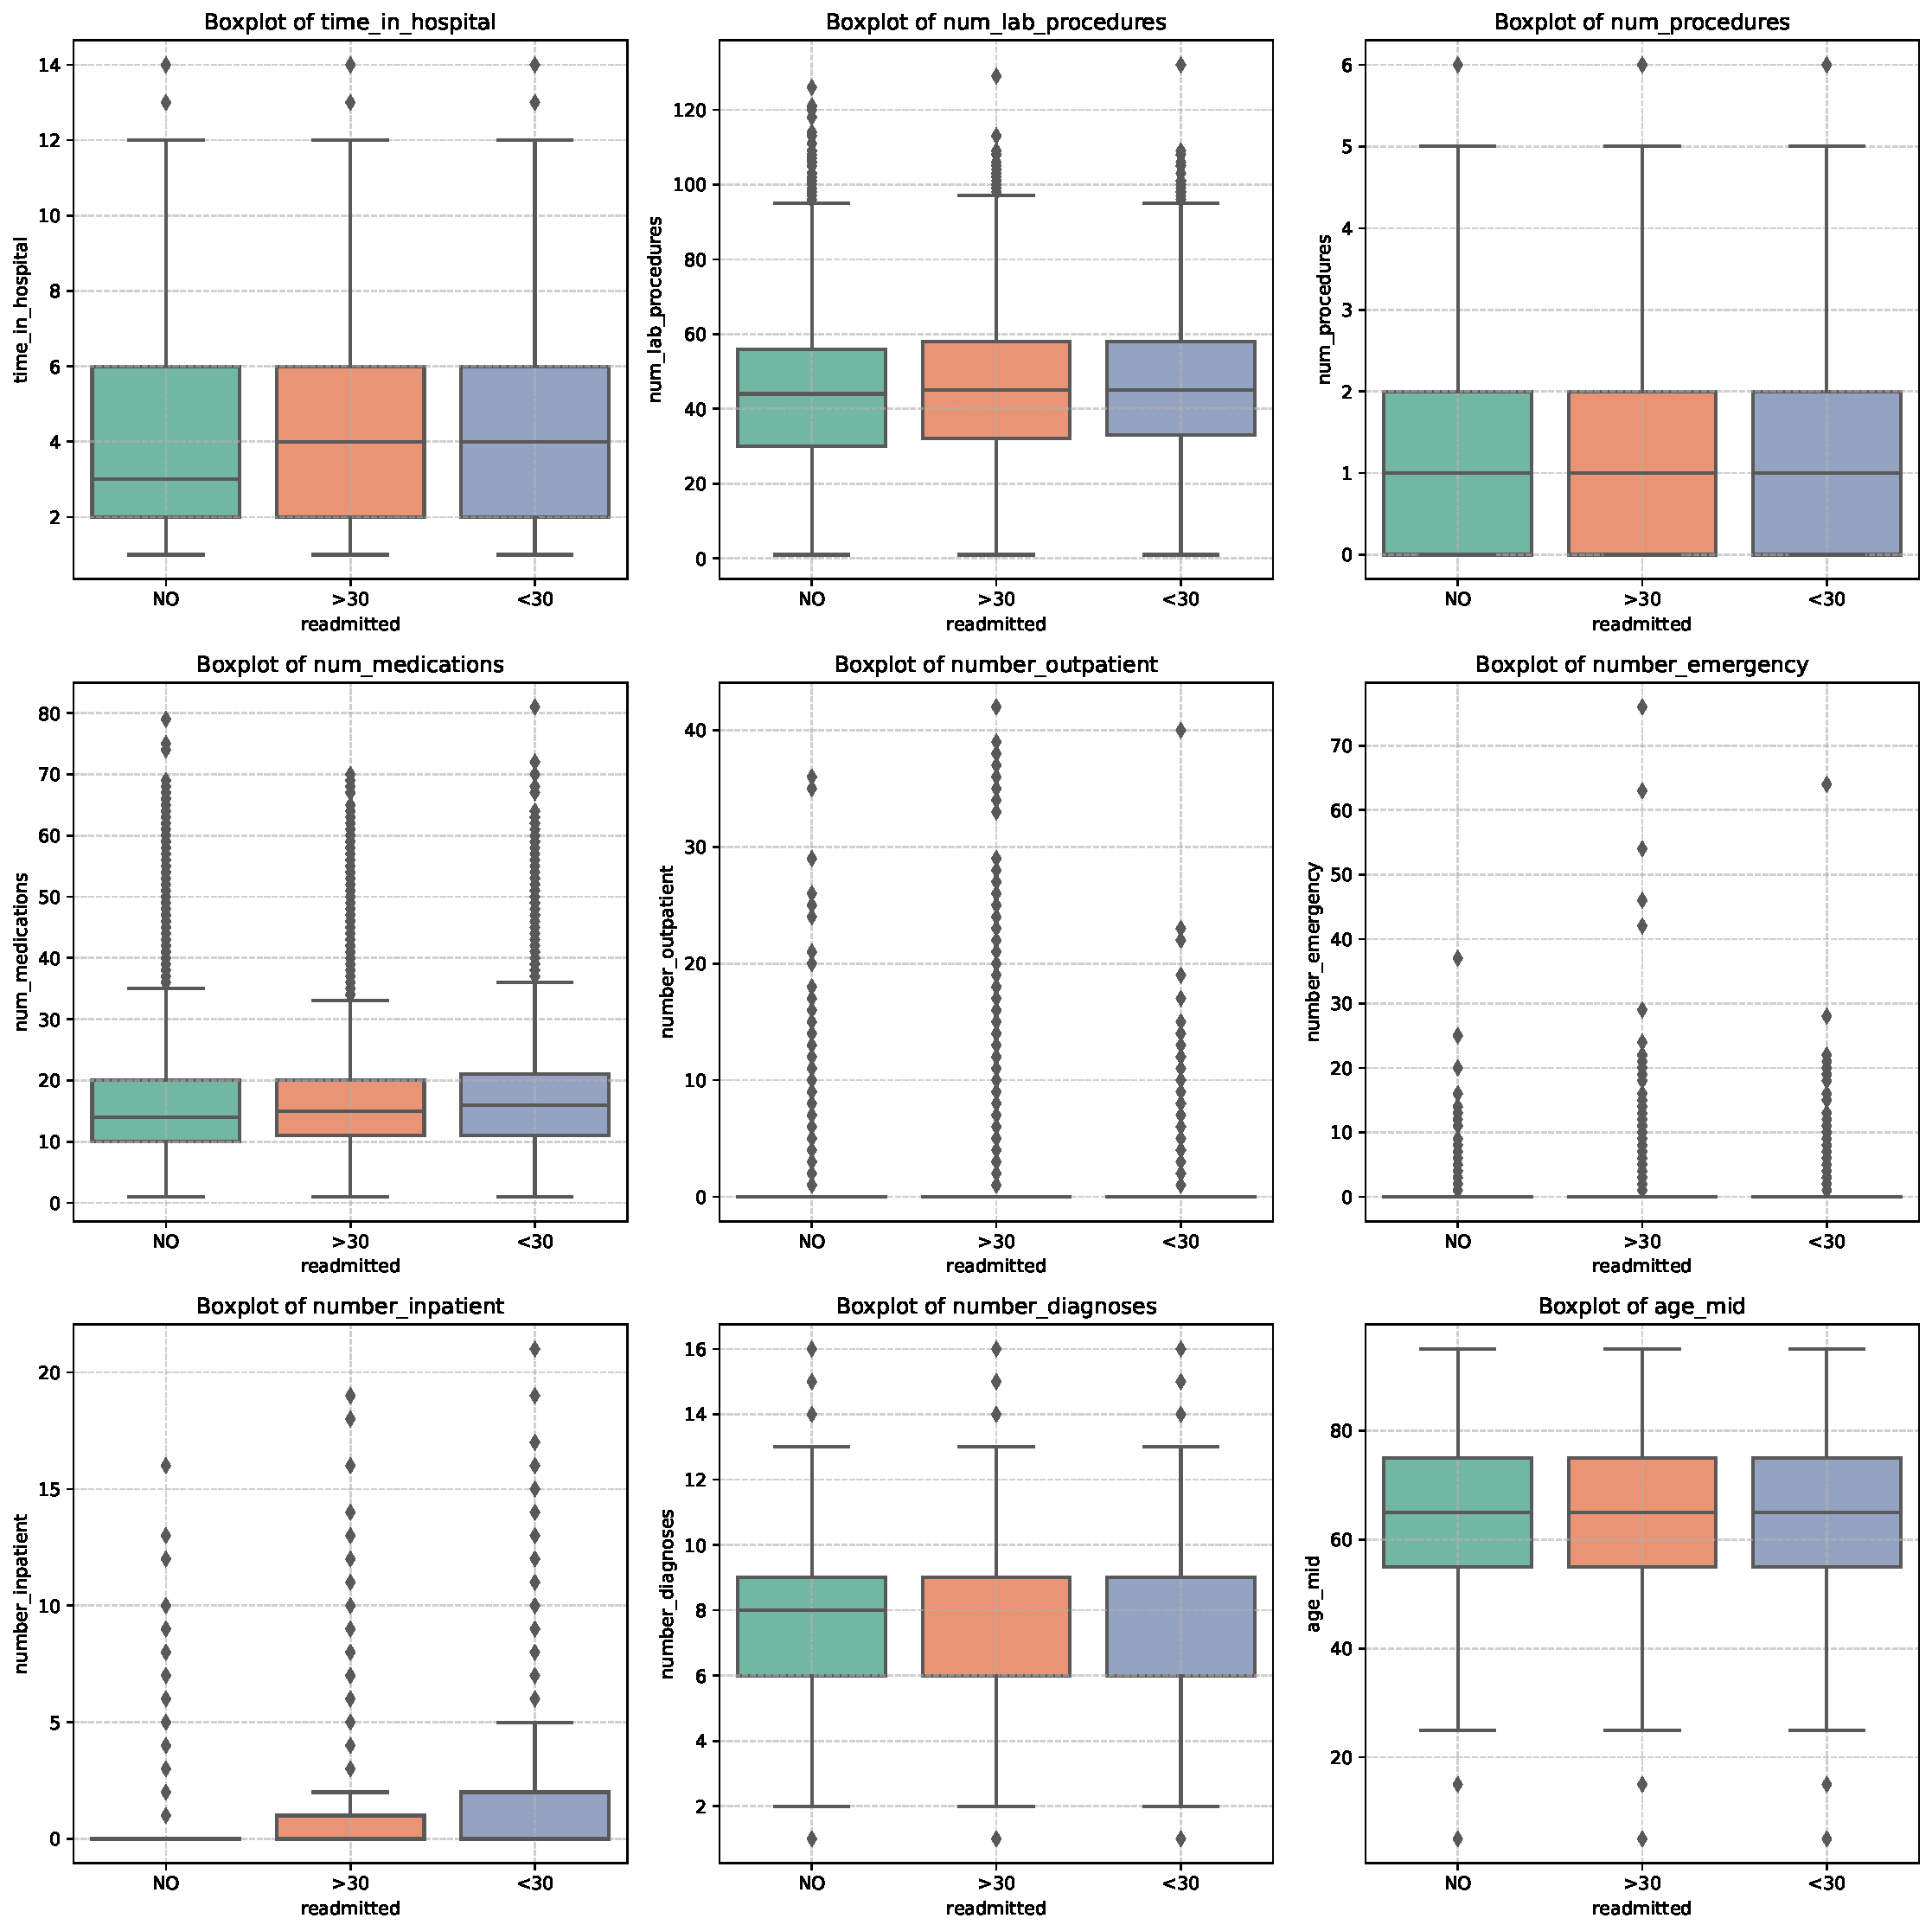
\includegraphics[width=0.9\textwidth]{../figures/numerical_boxplots.pdf}
    \caption{Boxplots of numerical variables by readmission status}
    \label{fig:num_boxplots}
\end{figure}

\section{Feature Engineering and Preparation for Modeling}

After comprehensive exploratory analysis, the following preprocessing steps were implemented to prepare the data for modeling:

\begin{enumerate}
    \item Merging of the transformed categorical variables (cat\_outpatient, cat\_emergency, cat\_inpatient) with the selected categorical features
    \item One-hot encoding of categorical variables, resulting in 193 binary features
    \item Standardization of remaining numerical variables
    \item Integration of encoded categorical features with standardized numerical features to form the final feature matrix
\end{enumerate}

This preprocessing pipeline transformed the original dataset with 50 variables into a modeling-ready matrix while preserving the information content and addressing the identified data quality issues.

\section{Feature Importance Analysis}

To gain deeper insights into the predictive power of individual features, a Random Forest classifier was trained on the preprocessed data. Feature importance scores were extracted to identify the most influential variables in predicting hospital readmission.

\begin{figure}[h]
    \centering
    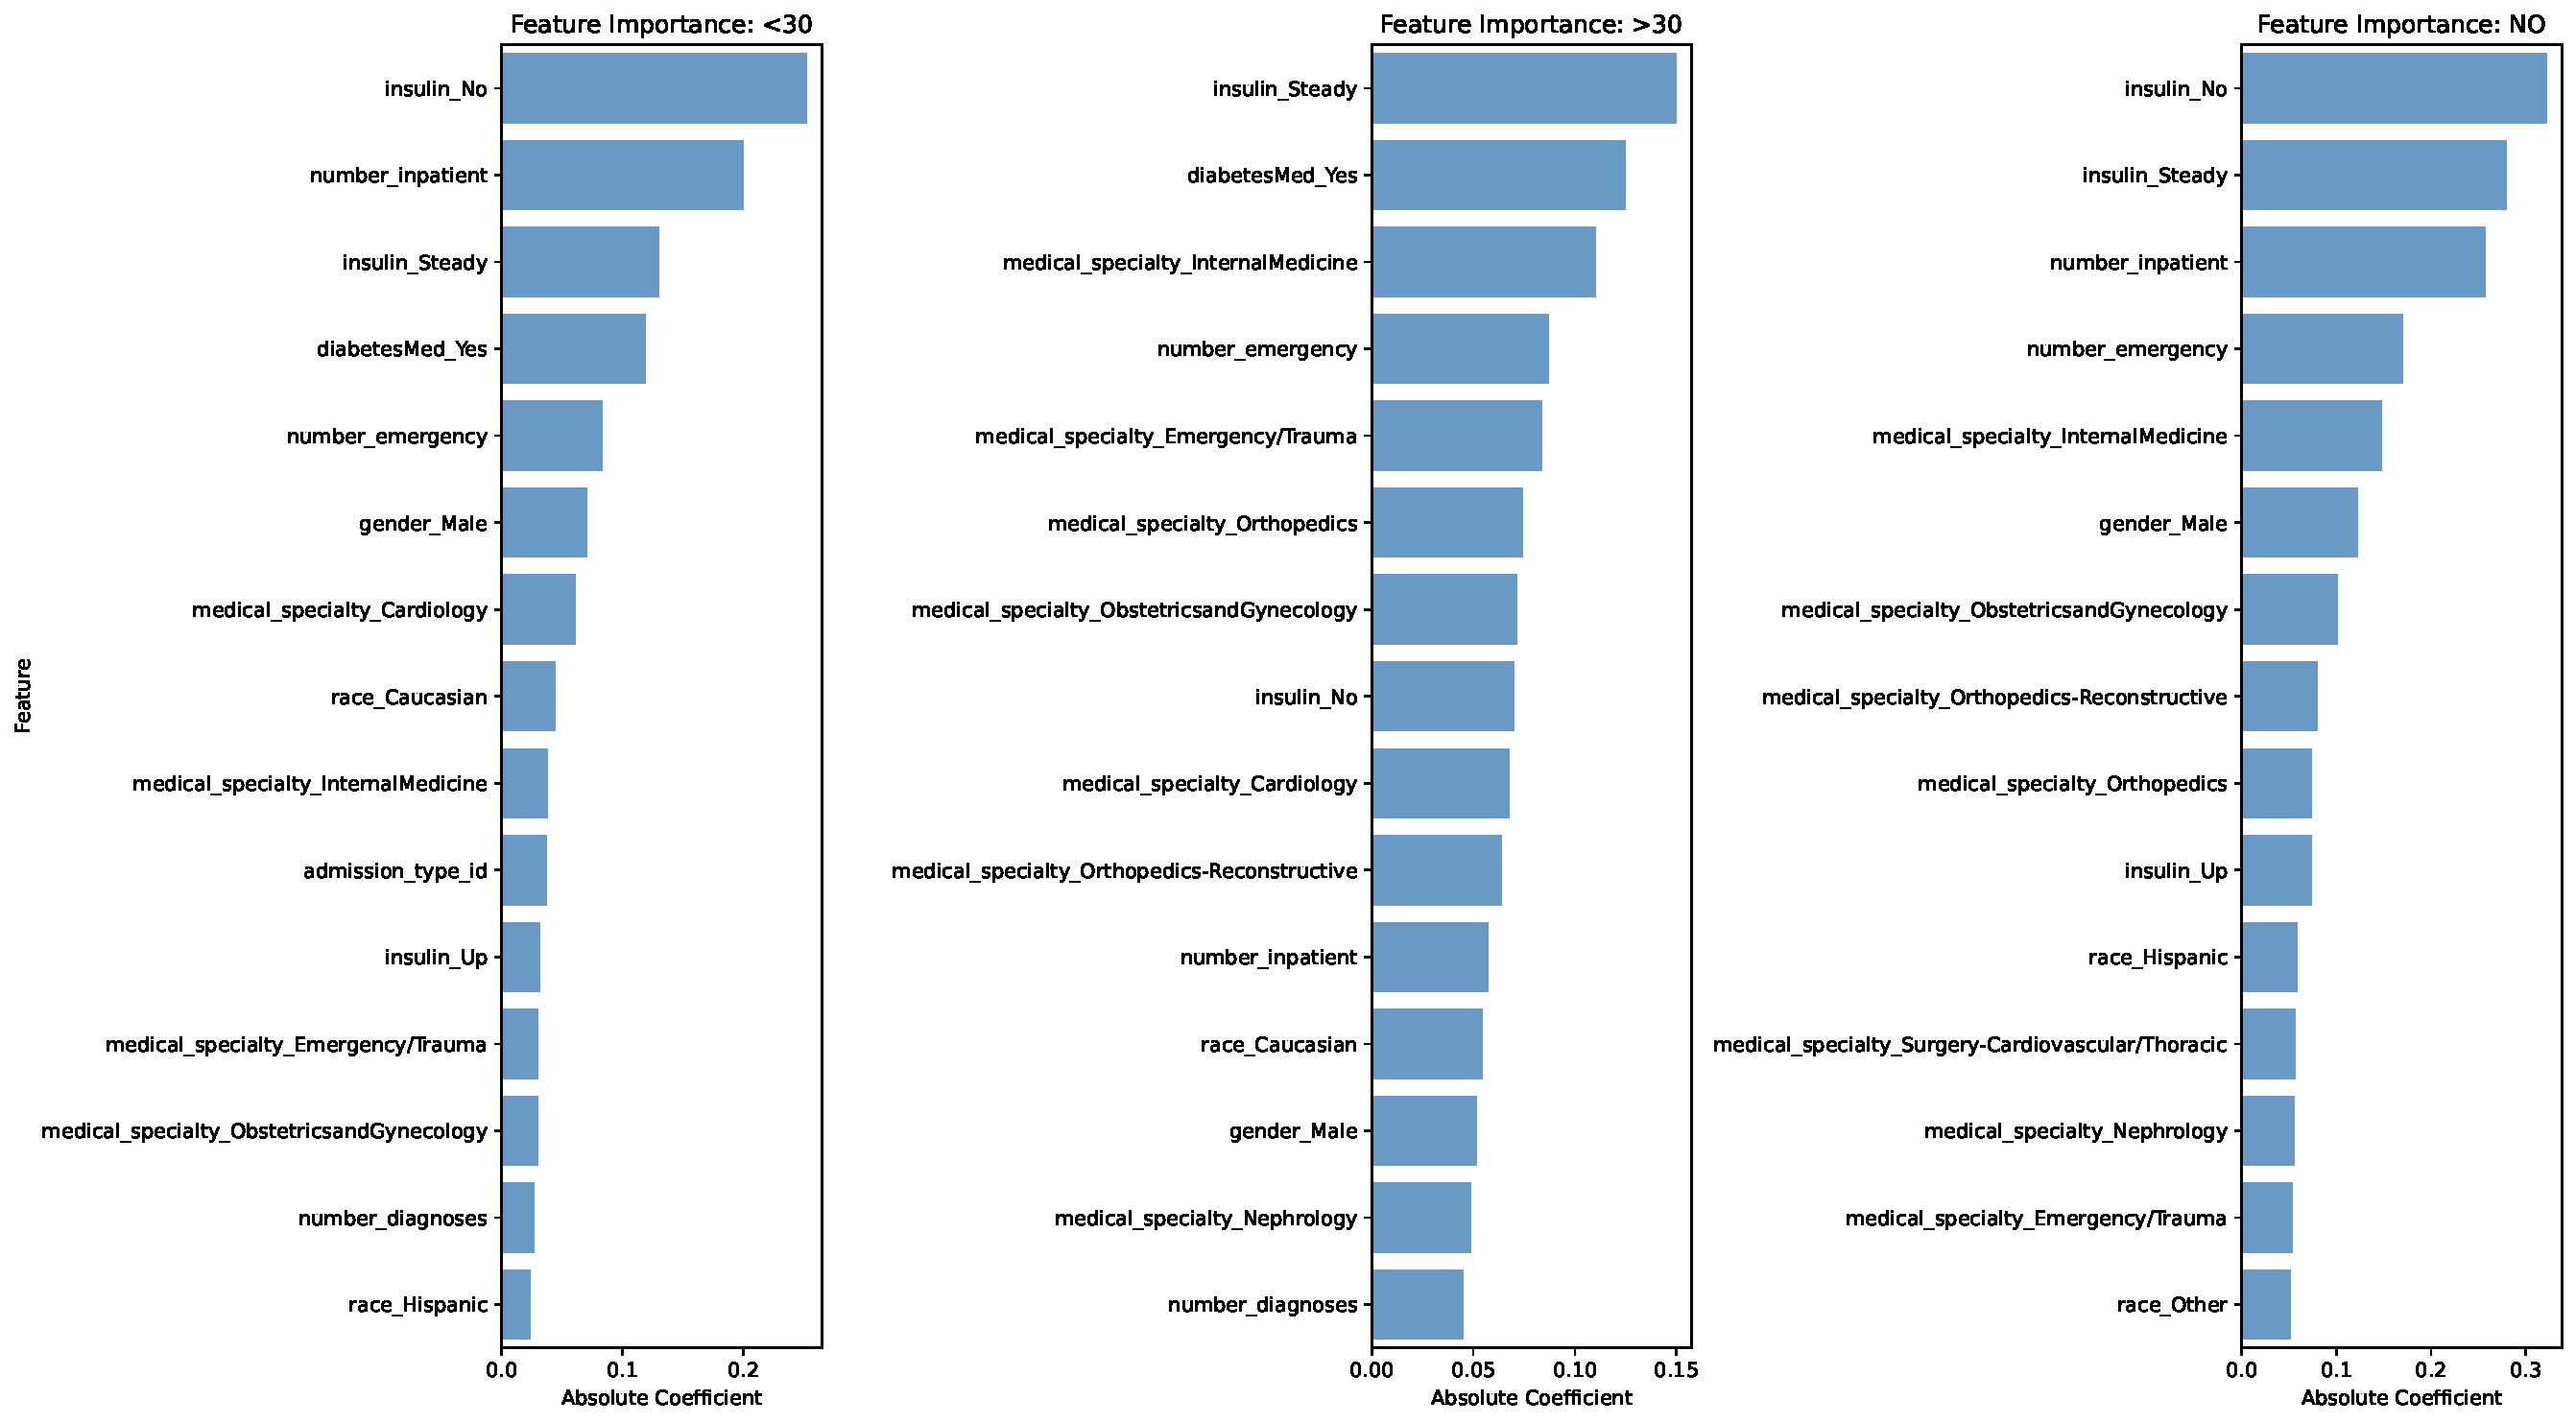
\includegraphics[width=0.9\textwidth]{../figures/feature_importance.pdf}
    \caption{Top 20 most important features based on Random Forest feature importance}
    \label{fig:feature_importance}
\end{figure}

The analysis revealed several key insights:
\begin{itemize}
    \item Hospital-related factors such as discharge\_disposition\_id and time\_in\_hospital emerged as the most important predictors of readmission
    \item Patient demographics including age and race also showed significant influence on readmission risk
    \item Clinical factors like number\_diagnoses, number\_inpatient visits, and number\_emergency visits were strong predictors
    \item Among medication variables, insulin treatment demonstrated the highest importance, supporting existing literature on the relationship between insulin therapy and readmission risk
\end{itemize}

These findings provide valuable insights for healthcare providers to identify high-risk patients and develop targeted interventions to reduce readmission rates. The prominence of hospital-related factors suggests that improvements in discharge planning and post-discharge follow-up could be effective strategies for reducing readmissions. 